% Build: cd report && pdflatex report.tex && pdflatex report.tex   (figures are read from ../results)
\documentclass[10pt,a4paper]{article}
\usepackage[margin=2.1cm]{geometry}
\usepackage[T1]{fontenc}
\usepackage{mathptmx}
\usepackage[scaled=0.9]{helvet}
\usepackage{courier}
\usepackage{microtype}
\usepackage{amsmath,amssymb}
\usepackage{booktabs}
\usepackage{tabularx}
\usepackage{graphicx}
\usepackage{xcolor}
\usepackage[font=small,labelfont=bf,skip=4pt]{caption}
\usepackage{enumitem}
\usepackage{titlesec}
\usepackage[numbers,sort&compress]{natbib}
\usepackage[colorlinks=true,linkcolor=blue!50!black,citecolor=blue!50!black,urlcolor=blue!50!black]{hyperref}

% Edit these three lines; everything else in report.tex stays unchanged.
\newcommand{\reportauthor}{AUTHOR NAME}
\newcommand{\reportaffil}{Independent research project}
\newcommand{\reportaiuse}{The code and much of the analysis were produced with an AI assistant (Claude, Anthropic) under the author's direction; the author ran all experiments and reviewed every result.}
   % defines \reportauthor and \reportaffil
\newcommand{\repo}{\url{https://github.com/sweetmAGIciaN7/mammography-multitask-ai}}
\graphicspath{{../results/}}
\titleformat{\section}{\sffamily\bfseries\large}{\thesection}{0.6em}{}
\titleformat{\subsection}{\sffamily\bfseries\normalsize}{\thesubsection}{0.6em}{}
\titlespacing*{\section}{0pt}{1.1em}{0.4em}
\titlespacing*{\subsection}{0pt}{0.8em}{0.3em}
\setlist{itemsep=1pt,topsep=3pt,leftmargin=1.4em}
\setlength{\parskip}{2pt}
\newcommand{\ci}[2]{\,{\footnotesize(#1 to #2)}}

\title{\sffamily\bfseries Augment, then split: a leakage-free replication of a\\multi-task attention model for mammography}
\author{\reportauthor\\{\small\reportaffil}}
\date{\small Technical report, \today\quad$\cdot$\quad Code and results: \repo}

\begin{document}
\maketitle

\begin{abstract}
\noindent Esen et al.\ (IEEE Access, 2025) propose a multi-task convolutional network with channel--spatial attention (CBAM)
that classifies mammograms as benign or malignant and grades breast density at the same time. They report 93.6\% accuracy
and an AUC of 0.962. I re-implemented the model and audited the evaluation. The paper's images were augmented into
$\sim$72 rotated and flipped copies \emph{before} the train/test split, and the reported accuracies are arithmetically
impossible on a test set of original images. Re-running that protocol on the same public data, the replication scores
a perfect AUC of 1.000; with a patient-level split it scores 0.755, and density prediction falls to the majority-class
baseline. On CBIS-DDSM (2,802 mammograms, 1,460 patients, biopsy-confirmed labels) with patient-level cross-validation,
the paper's design reaches AUC 0.782 (95\% CI 0.762--0.802), 0.746 on the official test split, and density agreement
QWK 0.769. Joint training gives no measurable benefit over single-task models, and CBAM adds a small +0.013 AUC.
Density grading transfers to an external digital dataset (INbreast, QWK 0.660), while calibration does not. Scored
against 376 radiologist-drawn lesion outlines, the CBAM ``attention map'' localises lesions barely better than a
lesion-blind brightness map (pointing game 0.24 vs 0.18). Grad-CAM of the same model does localise them (0.44). None of the
paper's attention statistics could be reproduced. The architecture is reasonable; the published numbers mostly measure
the evaluation protocol.
\end{abstract}

\begin{figure}[h]
\centering
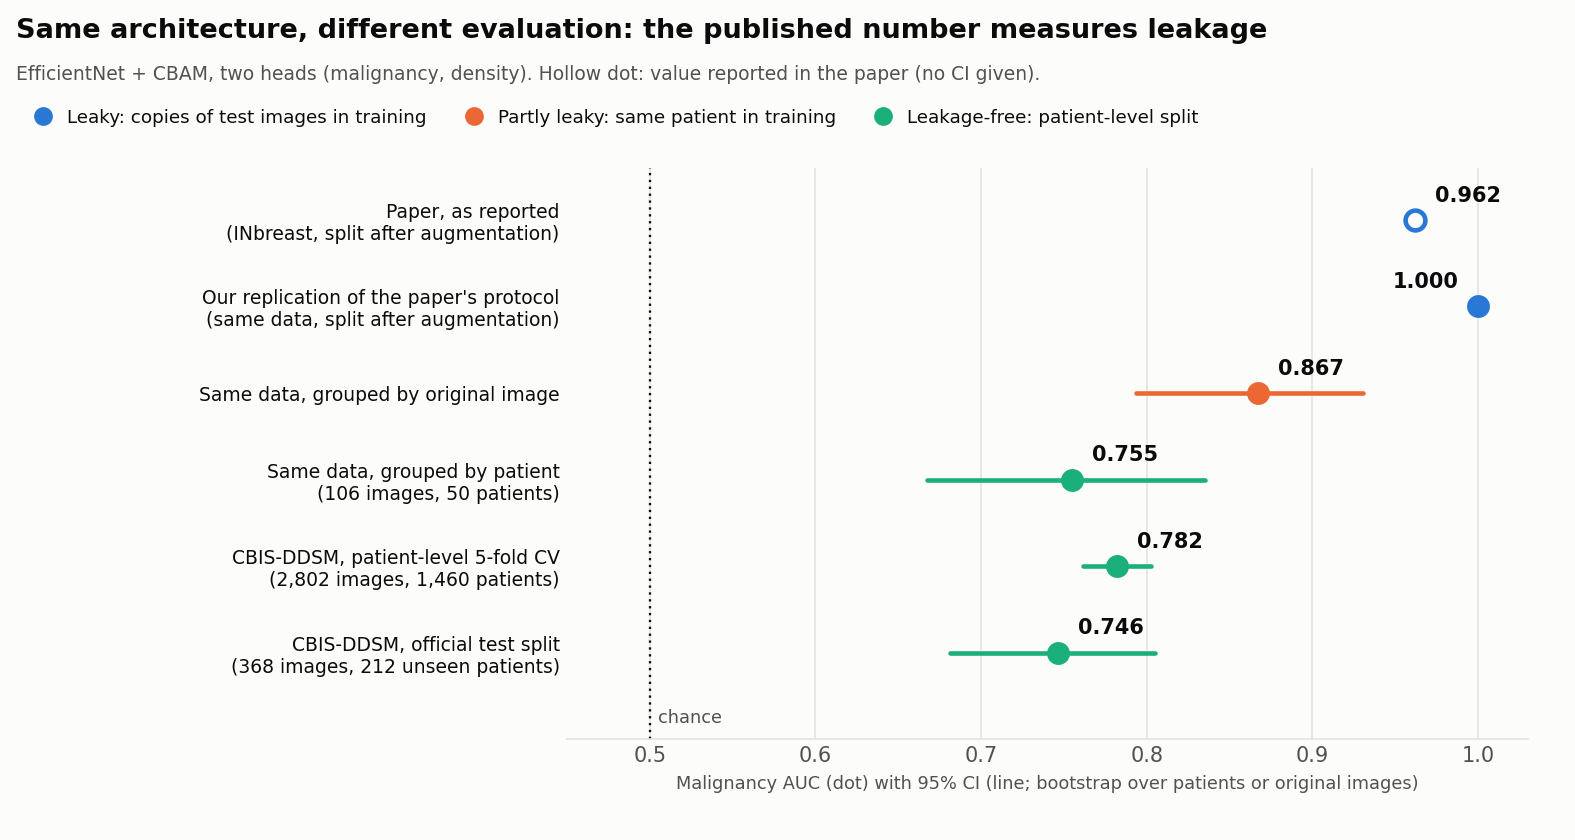
\includegraphics[width=0.92\linewidth]{overview/overview_chart.png}
\caption{Malignancy AUC of the same architecture under each evaluation protocol. Blue: the test set contains
augmented copies of training images. Orange: grouped by image, but other views of the same patient remain in
training. Green: no patient in both training and test. Lines are 95\% bootstrap CIs.}
\label{fig:overview}
\end{figure}

\section{Introduction}
Mammography screening generates large volumes of images, and deep-learning models that flag suspicious findings or
estimate breast density are an active research area. Breast density matters twice: dense tissue both hides tumours and
is an independent risk factor. A model that predicts malignancy \emph{and} density from one image is therefore
attractive, and multi-task learning~\cite{caruana1997} suggests that the two tasks might help each other.

Esen et al.~\cite{esen2025} build such a model: an EfficientNet backbone~\cite{tan2019}, a CBAM attention
module~\cite{woo2018} and two task heads. On INbreast~\cite{moreira2012} they report 93.6\% malignancy accuracy (AUC
0.962) and 88.9\% density accuracy, together with attention maps that ``strongly concentrate on irregular mass margins''.
My first re-implementation reached only 34--53\% accuracy. Instead of tuning until the numbers matched, I
examined how the paper evaluated its model and designed experiments to test each claim separately:
\begin{enumerate}[label=\textbf{Q\arabic*}]
\item Can the evaluation protocol alone explain the reported numbers? (Sec.~\ref{sec:leak})
\item With a leakage-free protocol, how good is the design, and do multi-task learning and attention help? (Sec.~\ref{sec:cbis})
\item Are the probabilities trustworthy, and does the model transfer to a different dataset? (Sec.~\ref{sec:cal}, \ref{sec:ext})
\item Do the attention maps actually point at lesions? (Sec.~\ref{sec:att})
\end{enumerate}
The critique is meant as a good-faith replication. Augment-then-split and patient overlap are common in medical
imaging~\cite{roberts2021,kapoor2023}, and nothing here implies intent.

\section{Audit of the reference evaluation}\label{sec:audit}
The full, itemised audit is in \texttt{PAPER\_AUDIT.md} in the repository. Its main points:
\begin{itemize}
\item \textbf{Augmentation before splitting.} Sec.~III-B states that every image was rotated to 11 angles and flipped,
and that ``subsequent to the augmentation process'' the data were split (Table~1: 7,208 augmented images). Fig.~1 cites
the Huang \& Lin dataset~\cite{huang2020}: 106 INbreast mass images augmented to 7,632 files in exactly the eight
density$\times$pathology folders of the paper's Table~1. The training set therefore almost certainly contains rotated
copies of every test mammogram.
\item \textbf{The accuracies need an augmented test set.} A 20\% hold-out of 410 images has 81--83 images. With
that many images the achievable accuracies near the reported values are 0.926--0.928 and 0.938--0.940. The reported
0.936 (hold-out) and 0.931/0.933/0.934 (cross-validation folds) cannot occur, so they must have been measured on
thousands of augmented files.
\item \textbf{Image-level split.} INbreast has 115 patients and 410 images; stratifying by image places the other views
of the same breast on both sides of the split.
\item \textbf{Brier score and ECE contradict each other.} For any binned calibration estimate, Jensen's inequality gives
$\mathrm{Brier}=\mathbb{E}[(p-y)^2]\ \ge\ \sum_b w_b(\bar p_b-\bar y_b)^2\ \ge\ \big(\sum_b w_b|\bar p_b-\bar y_b|\big)^2=\mathrm{ECE}^2$.
The reported pair (Brier 0.010, ECE 0.365--0.419) violates this bound by more than an order of magnitude.
\item \textbf{Other inconsistencies.} Table~1 rows sum to 7,328, not the stated 7,208. The ROC figure and the results
table give different AUCs for the same models. Two different attention architectures and three augmentation recipes
are described. Two of the four ``correct attention'' examples in Fig.~4 are misclassified.
\end{itemize}

\section{Methods}\label{sec:methods}
\paragraph{Data.} Three public datasets were used (Table~\ref{tab:data}). The Huang \& Lin set reproduces the paper's
setting for Q1. CBIS-DDSM~\cite{lee2017} gives biopsy-confirmed pathology for every finding, a BI-RADS density grade and
patient IDs. INbreast serves only as an external test set. CBIS-DDSM stores a mammogram twice when it contains both a
mass and calcifications. These 55 duplicates were merged (malignant if any finding is malignant). Patients listed in
both official CBIS-DDSM splits (22) were treated as training patients.

\begin{table}[h]
\centering\small
\caption{Datasets. ``Patients'' is the unit of every split and every bootstrap.}\label{tab:data}
\begin{tabularx}{\linewidth}{@{}lllX@{}}
\toprule
Dataset & Images / patients & Labels & Role \\
\midrule
Huang \& Lin~\cite{huang2020} & 106 originals $\times$ 72 copies / 50 & benign/malignant, density & Q1: leakage experiment \\
CBIS-DDSM~\cite{lee2017} & 2,802 / 1,460 (official test 368 / 212) & biopsy pathology, density & Q2--Q4: training, CV, test \\
INbreast~\cite{moreira2012} & 410 / 108 & density, BI-RADS (proxy) & Q3: external test only \\
\bottomrule
\end{tabularx}
\end{table}

\paragraph{Preprocessing.} Each mammogram is decoded at reduced resolution. The breast is cropped with an Otsu
threshold and the largest connected component. The image is flipped so the chest wall is on the left, then resized
with its aspect ratio kept to $640\times384$ pixels and zero-padded. INbreast DICOMs are first mapped to 8 bits with a
percentile window. The transform is recorded, so lesion masks can be sent through exactly the same geometry
(Sec.~\ref{sec:att}).

\paragraph{Model.} Fig.~\ref{fig:model} shows the replicated architecture (paper Sec.~IV-B). The loss is
$2.0\cdot\mathrm{BCE}_{\text{malignancy}}+0.8\cdot\mathrm{CE}_{\text{density}}$ with label smoothing 0.05, as in the paper.
I used EfficientNet-B0 rather than B3 and $640\times384$ rather than $224\times224$ input. Mammographic findings are
small, and B3 at full resolution was beyond the free GPU budget. Four variants share everything else:
\texttt{mt\_cbam} (paper design), \texttt{mt\_plain} (no CBAM), \texttt{st\_path} (malignancy head only) and
\texttt{st\_dens} (density head only). Training: AdamW (lr $2\cdot10^{-4}$, one-cycle schedule), 15 epochs, batch 16,
mixed precision, and augmentation that respects the chest-wall orientation (vertical flip, $\pm10^\circ$ rotation, zoom,
shift, brightness/contrast). There is no early stopping and no tuning on test folds.

\begin{figure}[t]
\centering
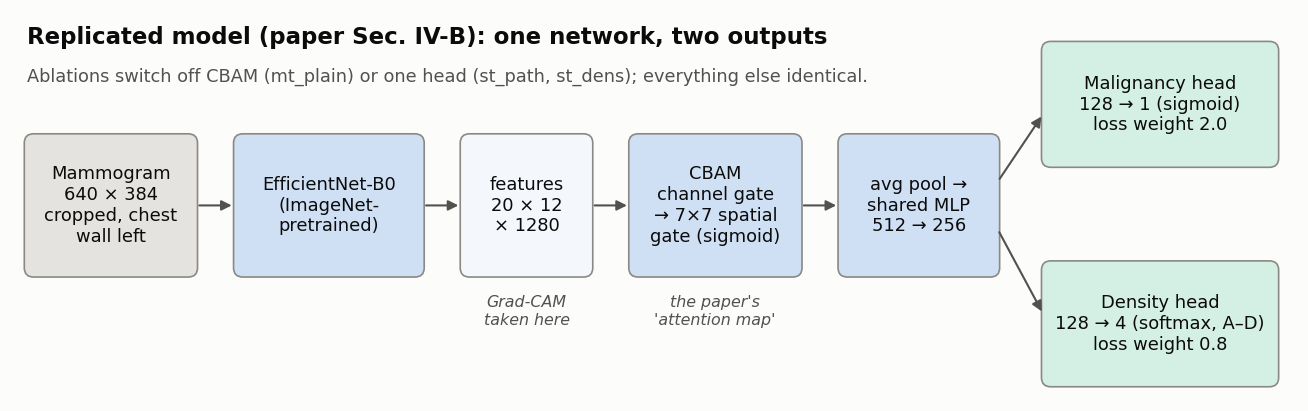
\includegraphics[width=\linewidth]{overview/model_diagram.png}
\caption{The replicated model. The CBAM spatial gate is what the paper calls the attention map. Grad-CAM is
computed on the backbone output, which is the same layer for every variant.}
\label{fig:model}
\end{figure}

\paragraph{Evaluation.} All splits are by patient and asserted to be disjoint. CBIS-DDSM uses 5-fold patient-level
cross-validation with identical folds for all variants; metrics are pooled over out-of-fold predictions. 95\%
confidence intervals come from a bootstrap over patients (2,000 resamples). Variants are compared with a \emph{paired}
bootstrap on the same test images. Density is scored with the quadratic-weighted kappa (QWK), which respects the
order A$<$B$<$C$<$D. Every metric is reported next to a majority-class baseline.

\section{Results}
\subsection{Q1: the leakage experiment}\label{sec:leak}
The paper-design model was trained three times on the Huang \& Lin files. Only the split changed: (i)~random over
files, as in the paper; (ii)~grouped by original image; (iii)~grouped by patient (5-fold CV, 8 epochs).

\begin{table}[h]
\centering\small
\caption{Q1. Same model, same data, only the split changes. Mean $\pm$ SD over 5 folds; pooled AUC with a cluster-bootstrap CI.}\label{tab:leak}
\begin{tabular}{@{}lcccc@{}}
\toprule
Split & Test patient also in training & Malignancy AUC & Pooled AUC (95\% CI) & Density acc. \\
\midrule
Paper protocol (augment, then split) & 100\% & $1.000\pm0.000$ & 1.000 & 1.000 \\
Grouped by original image & 97\% & $0.867\pm0.066$ & 0.867\ci{0.794}{0.931} & 0.689 \\
Grouped by patient & 0\% & $0.724\pm0.093$ & 0.755\ci{0.667}{0.835} & 0.403 \\
\emph{Majority class} & & 0.500 & & 0.401 \\
\bottomrule
\end{tabular}
\end{table}

The paper's protocol yields a perfect score, higher than the paper's own 0.962, because on average 57 of each
test file's 71 siblings are in training. Grouping by image is not enough: 97\% of test images still had a
different view of the same patient in training. With a patient-level split, malignancy AUC falls to 0.72--0.76, and
density accuracy (0.403) equals the majority-class rate (0.401). With leakage, the model had learned to recognise
\emph{patients}, not density.

\subsection{Q2: a leakage-free multi-task model on CBIS-DDSM}\label{sec:cbis}
\begin{table}[h]
\centering\small
\caption{Q2. CBIS-DDSM, patient-level 5-fold CV, pooled out-of-fold (2,802 images, 1,460 patients). 95\% CIs by patient bootstrap.}\label{tab:cbis}
\begin{tabular}{@{}lcccc@{}}
\toprule
Variant & Malignancy AUC & Malignancy acc. & Density acc. & Density QWK \\
\midrule
\texttt{mt\_cbam} (paper design) & \textbf{0.782}\ci{0.762}{0.802} & 0.700 & 0.668 & 0.769\ci{0.746}{0.791} \\
\texttt{mt\_plain} (no attention) & 0.769\ci{0.748}{0.789} & 0.697 & 0.653 & 0.761\ci{0.735}{0.784} \\
\texttt{st\_path} (malignancy only) & 0.773\ci{0.752}{0.793} & 0.691 & -- & -- \\
\texttt{st\_dens} (density only) & -- & -- & 0.681 & \textbf{0.780}\ci{0.755}{0.802} \\
\emph{Majority class} & 0.500 & 0.552 & 0.395 & 0.000 \\
\bottomrule
\end{tabular}
\end{table}

With an honest split the design reaches AUC 0.782 (Table~\ref{tab:cbis}), within the range usually seen for
whole-image classification of downsampled mammograms. On the official test split (368 images, 212 unseen patients),
a single model trained on the official training patients reaches AUC 0.746\ci{0.681}{0.805} and QWK 0.711\ci{0.631}{0.773}.
Paired comparisons:
\begin{itemize}
\item adding the density task to malignancy: $\Delta$AUC $+0.009$\ci{$-0.004$}{$+0.024$}, no clear effect;
\item adding the malignancy task to density: $\Delta$QWK $-0.010$\ci{$-0.026$}{$+0.005$}, no clear effect;
\item adding CBAM for malignancy: $\Delta$AUC $+0.013$\ci{$+0.002$}{$+0.026$}. This is a small gain from a single training seed, below the fold-to-fold spread ($\pm0.025$);
\item adding CBAM for density: $\Delta$QWK $+0.008$\ci{$-0.005$}{$+0.023$}.
\end{itemize}
Performance depends on the lesion type: AUC 0.83 on images with masses and 0.72 on images with only calcifications,
which are a few pixels across at this resolution. CC and MLO views score the same (0.78).

\begin{figure}[t]
\centering
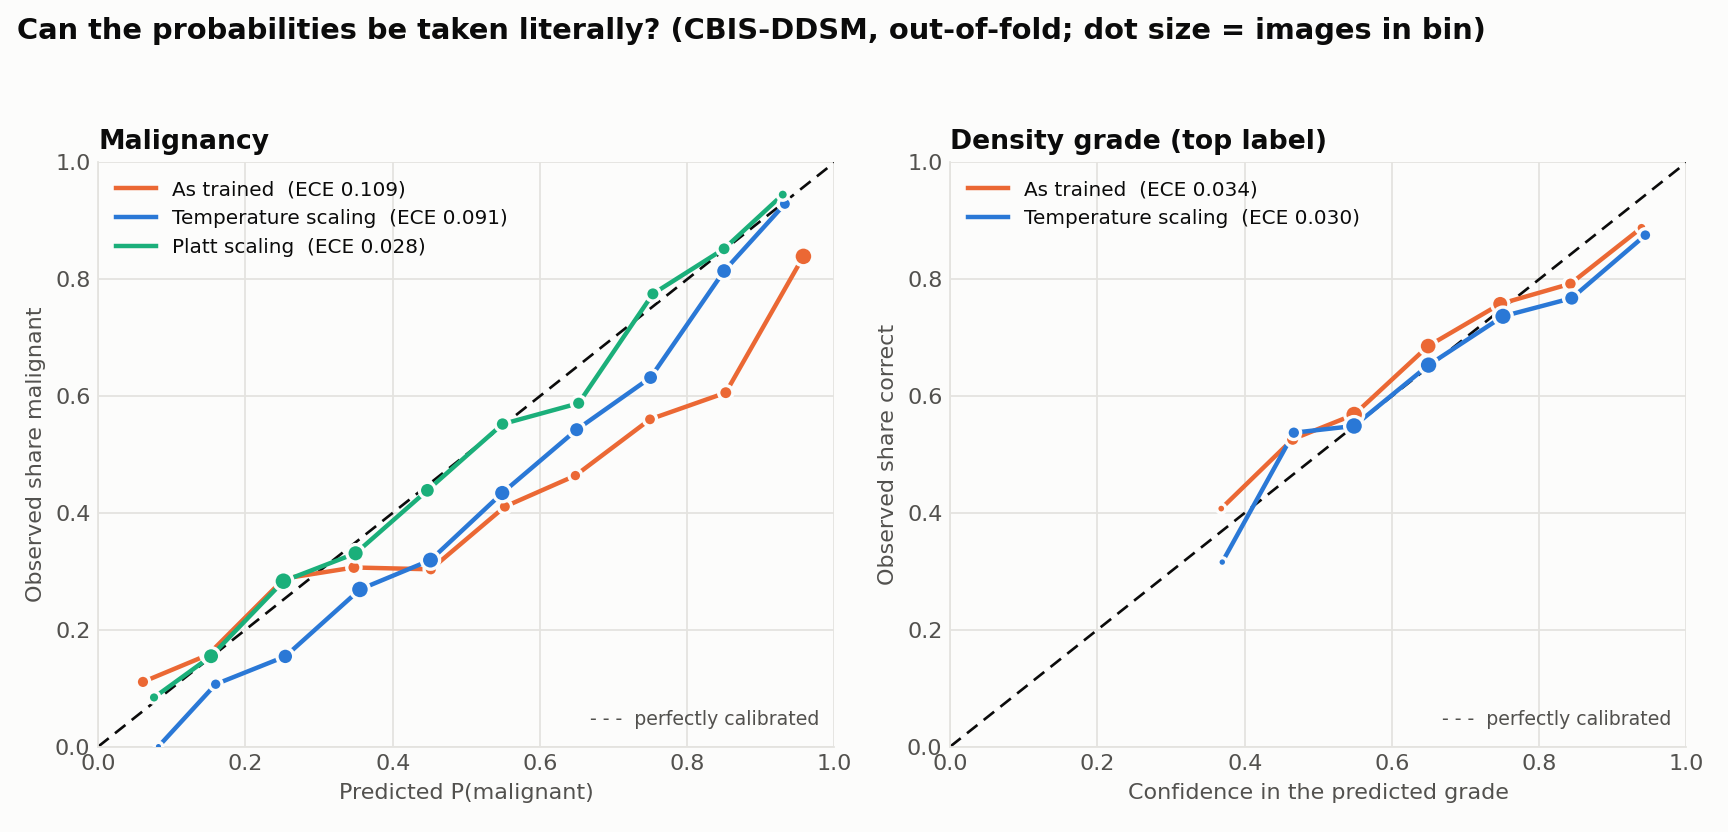
\includegraphics[width=0.62\linewidth]{calibration/reliability_diagram.png}
\caption{Q3a. Reliability of the malignancy output and of the density grade (cross-validation, out-of-fold),
before and after cross-fitted temperature and Platt scaling.}
\label{fig:cal}
\end{figure}

\subsection{Q3a: calibration and operating points}\label{sec:cal}
A model can rank cases well and still give misleading probabilities (Fig.~\ref{fig:cal}). Using the cross-validation
out-of-fold predictions of Table~\ref{tab:cbis}, every calibration map was fitted on four folds and applied to the fifth.
\begin{itemize}
\item The raw malignancy output is over-confident \emph{and} biased: its mean prediction is 0.542 against a true rate
of 0.448, and ECE is 0.109 (95\% CI 0.095--0.131).
\item Temperature scaling~\cite{guo2017} (T$\approx$1.74) only softens the probabilities (ECE 0.091). Platt
scaling~\cite{platt1999}, which also has an intercept, removes the bias: ECE 0.028, Brier 0.205$\to$0.188.
\item The density head is already calibrated (top-label ECE 0.034).
\item The parameters transfer only partly to a separately trained model: on the official-split model, ECE drops from
0.206 to 0.090.
\item A threshold chosen on the other folds for 90\% sensitivity reached 89.8\% on unseen patients, with specificity
0.386.
\end{itemize}
The sensitivity/specificity trade-off is set by this threshold. The paper claims that its loss weights
``ensure minimizing false negatives'', but the relative weight of two task losses does not set that trade-off. All our
models satisfy Brier $\ge$ ECE$^2$.

\subsection{Q3b: external validation on INbreast}\label{sec:ext}
The four official-split models were applied unchanged to all 410 INbreast images, which are full-field digital
mammograms from Portugal (Fig.~\ref{fig:ext}). The training data are scanned US film from the 1990s.

\begin{figure}[t]
\centering
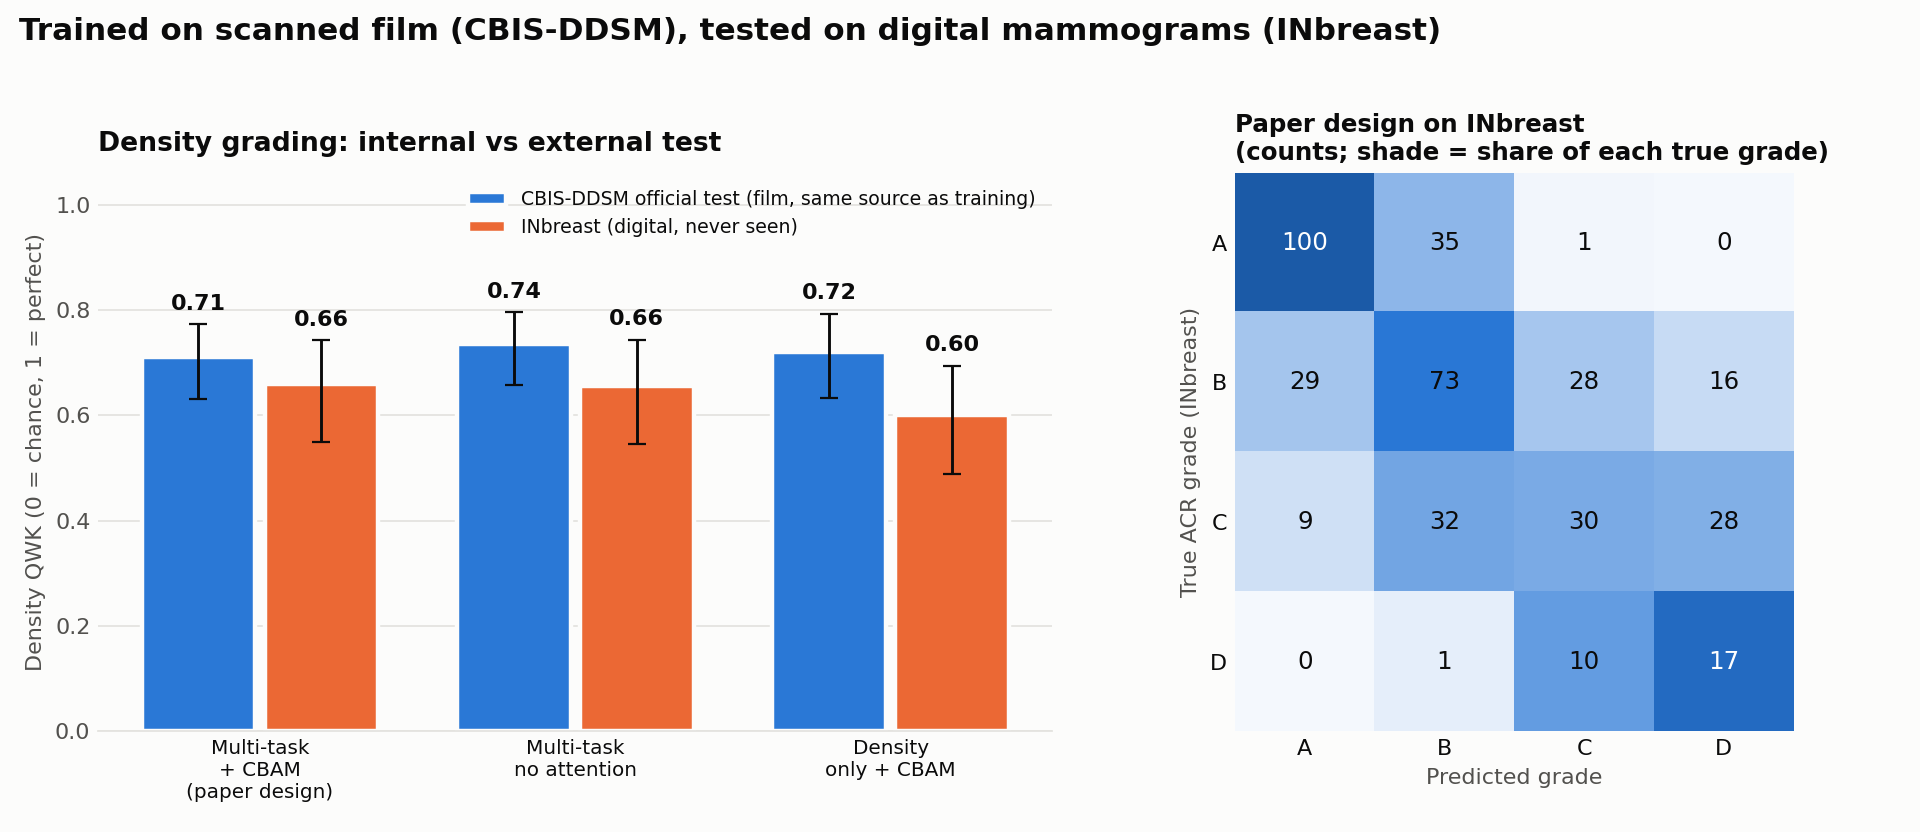
\includegraphics[width=\linewidth]{external/external_chart.png}
\caption{Q3b. Density grading on the internal (CBIS-DDSM official test) and external (INbreast) test sets for each
variant, with 95\% CIs (bootstrap over patients), and the paper design's confusion matrix on INbreast.}
\label{fig:ext}
\end{figure}
\begin{itemize}
\item \textbf{Density transfers.} QWK is 0.660\ci{0.550}{0.743} against 0.711 in-domain. 93.4\% of predictions are
within one grade of the radiologist's. The majority-class accuracy is 0.357; the model reaches 0.538. It over-calls
the densest grade (61 predicted D vs 28 true).
\item \textbf{Malignancy, on a proxy.} INbreast has no biopsy label for most images, so the target is BI-RADS 4--6
vs 1--3. The AUC is 0.822\ci{0.761}{0.877}, and the mean score rises steadily with BI-RADS: 0.25, 0.28, 0.28, 0.43,
0.75, 0.79. This task is easier than CBIS-DDSM's, because it includes normal mammograms.
\item \textbf{Calibration does not transfer.} The two multi-task variants rank images similarly, but on normal
INbreast images they predict 0.25 and 0.54 on average. The CBIS temperature makes density ECE slightly worse
(0.107$\to$0.129).
\item Multi-task vs single-task density: $\Delta$QWK $+0.059$\ci{$-0.019$}{$+0.146$}. This suggests but does not show
better transfer.
\end{itemize}

\subsection{Q4: do the attention maps point at the lesion?}\label{sec:att}
The paper supports its interpretability claims with four hand-picked images and statistics without a stated method.
I scored the CBAM gate and Grad-CAM~\cite{selvaraju2017} of the official-split models on the official CBIS-DDSM test split against the radiologists' ROI masks.
Masks were identified by content, since CBIS-DDSM sometimes swaps its crop and mask files, and sent through each image's own
crop, flip and resize: 376 of 390 findings, on 354 images from 206 patients. Maps are $20\times12$ (stride 32). Metrics
are computed inside the breast:
\begin{itemize}
\item the pointing game~\cite{zhang2018}: the map's maximum lies on the lesion, within one cell;
\item energy in lesion: the share of the map's mass on the lesion;
\item pixel AUC: lesion vs other breast pixels.
\end{itemize}
Lesion-blind baselines (uniform, random, brightest tissue, breast centre) and an ImageNet-only network define what
``better than chance'' means.

\begin{figure}[t]
\centering
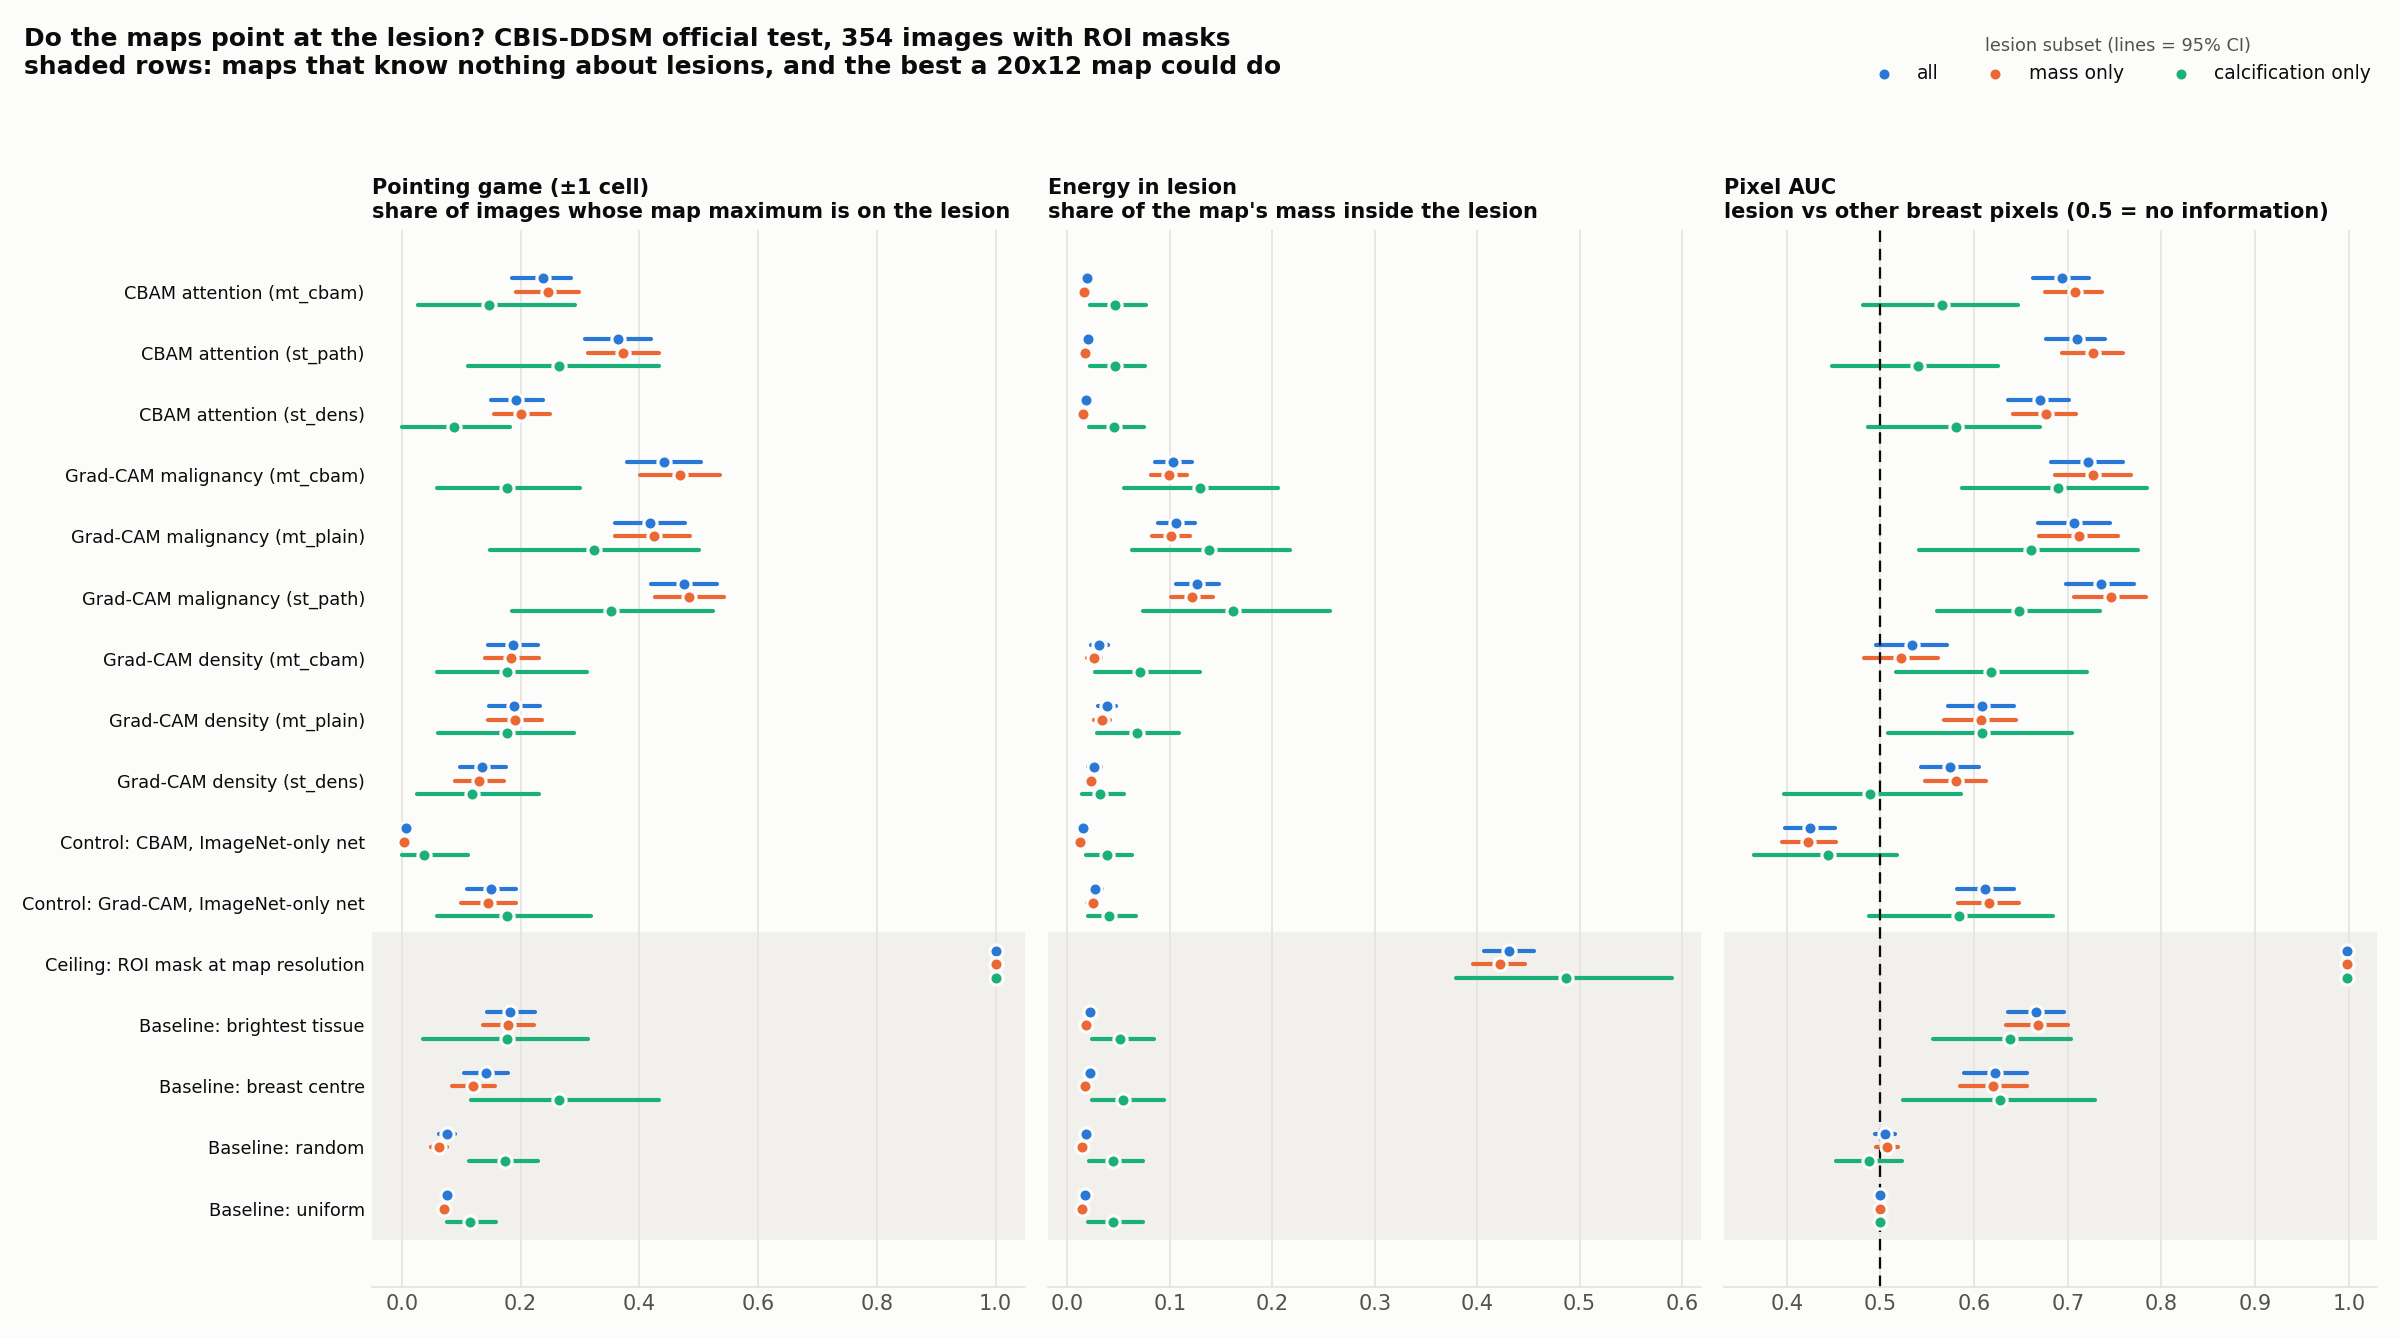
\includegraphics[width=\linewidth]{attention/localisation_chart.png}
\caption{Q4. Pointing game ($\pm$1 cell) and energy in lesion for each map, with 95\% CIs (patient bootstrap), next to
lesion-blind baselines and the ceiling (the ROI mask itself at map resolution).}
\label{fig:att}
\end{figure}

\begin{table}[h]
\centering\small
\caption{Q4. Localisation on 354 official-test images (95\% CI, patient bootstrap). Chance energy $=$ the lesion's share of the breast (0.018).}\label{tab:att}
\begin{tabular}{@{}lccc@{}}
\toprule
Map & Pointing ($\pm$1 cell) & Energy in lesion & Pixel AUC \\
\midrule
CBAM gate, paper design & 0.24\ci{0.19}{0.29} & 0.019\ci{0.016}{0.024} & 0.69\ci{0.66}{0.72} \\
Grad-CAM (malignancy), paper design & \textbf{0.44}\ci{0.38}{0.50} & \textbf{0.103}\ci{0.085}{0.121} & 0.72\ci{0.68}{0.76} \\
Grad-CAM (malignancy), no-attention model & 0.42\ci{0.36}{0.48} & 0.106 & 0.71 \\
Grad-CAM (density), paper design & 0.19 & 0.031 & 0.53 \\
\emph{ImageNet-only network, Grad-CAM} & 0.15 & 0.028 & 0.61 \\
\emph{Brightest tissue} & 0.18\ci{0.14}{0.22} & 0.022 & 0.67 \\
\emph{Uniform (chance)} & 0.08 & 0.018 & 0.50 \\
\emph{Ceiling: ROI mask at $20\times12$} & 1.00 & 0.431 & 1.00 \\
\bottomrule
\end{tabular}
\end{table}

The CBAM gate is \emph{open almost everywhere}: its mean value is 0.85, and its normalised entropy is 0.995. It beats the
brightness baseline by only $+0.055$ (0.000 to $+0.108$) on pointing, and its energy on the lesion equals chance. A
min--max-scaled heatmap of such a gate can still \emph{look} focused. Grad-CAM of the same model points at the lesion
in 44\% of images (66\% of malignant ones) and puts 5.7$\times$ chance energy on it. The ImageNet-only control scores
0.15, so the localisation comes from training on mammograms. CBAM does not improve Grad-CAM localisation ($+0.023$,
$-0.017$ to $+0.061$). Lesions smaller than one cell are found far less often (0.29 vs 0.56 for 1--4 cells).

Using explicit definitions on the map pooled to the paper's $7\times7$ grid, none of the paper's statistics
was reproduced:
\begin{itemize}
\item Gini, malignant vs benign: 0.088 vs 0.081 (paper 0.68 vs 0.43);
\item entropy: 3.876 vs 3.879 nats, both 99.6\% of the maximum $\ln 49$ (paper 2.31 vs 3.74; the paper's ``benign''
value is itself 96\% of the maximum);
\item peak attention, dense vs non-dense: 0.999 vs 0.999, $r=+0.02$ (paper 0.82 vs 0.61, $r=0.61$);
\item 80\%-mass area: 75\% vs 75\% (paper 12\% vs 29\%).
\end{itemize}

\section{Discussion}
\paragraph{What the design is worth.} With an honest evaluation the multi-task CBAM network is a solid baseline: AUC
0.75--0.78 for whole-image malignancy on CBIS-DDSM, good density agreement, and density grading that survives a change
of country and imaging technology. Its selling points are not supported. Multi-task training does not improve either
task measurably. It saves one network, which is a real but modest benefit. The attention gate adds little accuracy and
no interpretability. Where explanations are needed, Grad-CAM on the same model is the better tool, although it too
misses more than half the lesions at this resolution.

\paragraph{Why the gap matters.} The difference between 0.96 and 0.75--0.78 is not a detail. A reader of the paper
would expect a model close to clinical performance and a working lesion localiser; neither holds. The cause is a
single ordering decision, augmenting before splitting, combined with an image-level split on a dataset of 50 patients.
Both are cheap to avoid: split by patient first, augment only the training set, and report a majority baseline and a
confidence interval with every metric.

\paragraph{Limitations.}
\begin{itemize}
\item \textbf{One seed per model.} Effects of about 0.01 AUC (CBAM) are not established.
\item \textbf{Not the paper's exact setup.} The backbone and resolution differ, and the paper's data and splits are
unreleased, so Q1 relies on the dataset the paper cites.
\item \textbf{Findings, not screening.} CBIS-DDSM contains only images with findings, so these results say nothing
about screening performance.
\item \textbf{Small and uneven test data.} The external set is small (108 patients) and uses a BI-RADS proxy for
malignancy. Calcifications are under-represented in the localisation test (34 images), and their outlines are loose.
\end{itemize}

\section{Conclusion}
Reproducing a published medical-imaging result required auditing its evaluation first. The reported 93.6\%
accuracy is explained by the paper's protocol: the same model on the same data scores 100\% under that protocol and
about 75\% without leakage. Evaluated properly, the architecture is useful but ordinary, and its attention maps do not
show what the paper says they show. All code, per-image predictions, figures and a demo are public.

\paragraph{Reproducibility and AI assistance.} Every experiment is one script and one free Kaggle notebook. Retraining
with the same seed reproduced the official-split results to three decimals. Unit tests check the split logic,
preprocessing geometry and metrics. \reportaiuse

\small
\begin{thebibliography}{99}
\bibitem[Esen et~al.(2025)]{esen2025} G.~Esen, M.~Nurtas, L.~La Paglia, J.~Amankulov, B.~Matkerim, A.~Altaibek.
Multi-task attention-guided deep learning for simultaneous breast cancer detection and density estimation in
mammography. \emph{IEEE Access}, 13:198938--198951, 2025. doi:10.1109/ACCESS.2025.3634473.
\bibitem[Caruana(1997)]{caruana1997} R.~Caruana. Multitask learning. \emph{Machine Learning}, 28:41--75, 1997.
\bibitem[Tan and Le(2019)]{tan2019} M.~Tan, Q.~V.~Le. EfficientNet: rethinking model scaling for convolutional neural
networks. In \emph{ICML}, 2019.
\bibitem[Woo et~al.(2018)]{woo2018} S.~Woo, J.~Park, J.-Y.~Lee, I.~S.~Kweon. CBAM: convolutional block attention
module. In \emph{ECCV}, 2018.
\bibitem[Moreira et~al.(2012)]{moreira2012} I.~C.~Moreira et~al. INbreast: toward a full-field digital mammographic
database. \emph{Academic Radiology}, 19(2):236--248, 2012.
\bibitem[Lee et~al.(2017)]{lee2017} R.~S.~Lee et~al. A curated mammography data set for use in computer-aided detection
and diagnosis research. \emph{Scientific Data}, 4:170177, 2017.
\bibitem[Huang and Lin(2020)]{huang2020} M.-L.~Huang, T.-Y.~Lin. Dataset of breast mammography images with masses.
\emph{Data in Brief}, 31:105928, 2020.
\bibitem[Roberts et~al.(2021)]{roberts2021} M.~Roberts et~al. Common pitfalls and recommendations for using machine
learning to detect and prognosticate for COVID-19 using chest radiographs and CT scans. \emph{Nature Machine
Intelligence}, 3:199--217, 2021.
\bibitem[Kapoor and Narayanan(2023)]{kapoor2023} S.~Kapoor, A.~Narayanan. Leakage and the reproducibility crisis in
machine-learning-based science. \emph{Patterns}, 4(9):100804, 2023.
\bibitem[Guo et~al.(2017)]{guo2017} C.~Guo, G.~Pleiss, Y.~Sun, K.~Q.~Weinberger. On calibration of modern neural
networks. In \emph{ICML}, 2017.
\bibitem[Platt(1999)]{platt1999} J.~Platt. Probabilistic outputs for support vector machines and comparisons to
regularized likelihood methods. In \emph{Advances in Large Margin Classifiers}, 1999.
\bibitem[Selvaraju et~al.(2017)]{selvaraju2017} R.~R.~Selvaraju et~al. Grad-CAM: visual explanations from deep
networks via gradient-based localization. In \emph{ICCV}, 2017.
\bibitem[Zhang et~al.(2018)]{zhang2018} J.~Zhang et~al. Top-down neural attention by excitation backprop.
\emph{International Journal of Computer Vision}, 126:1084--1102, 2018.
\end{thebibliography}
\end{document}
